\section{Introduction}
The interest for application-specific hardware is growing in different fields of computer science, from embedded to High Performance Computing systems. This is mostly due to the end of Dennard Scaling~\cite{esmaeilzadeh2011dark}
%ADDCITATION ((2013). The End of Dennard Scaling. Accessed: Feb. 2013. [Online].
%Available: https://cartesianproduct.wordpress.com/2013/04/15/the-endof-dennard-scaling/
%[3] H. Esmaeilzadeh, E. Blem, R. S. Amant, K. Sankaralingam, and
%D. Burger, “Dark silicon and the end of multicore scaling,” in Proc.
%38th Annu. Int. Symp. Comput. Archit. (ISCA), Jun. 2011, pp. 365–376.}
and the ever increasing demand for performance and lower power consumption. Application-specific or \textit{custom processor} hardware seems to be the solution to face current silicon challenges allowing energy savings and performance increase over general purpose counterparts~\cite{hameed2010understanding}. With the massive increase in the data handling needed in custom hardware, the \textit{memory system} (both on-chip and off-chip) is becoming a dominant factor affecting the overall performance, power consumption and area usage of the silicon. Since the memory system and the processing system are strongly \textit{interdependent}, they should be \textit{co-designed}. This is especially important for emerging memory technologies, such as MRAM, eDRAM, PCM, RRAM~\cite{mem2016}, that has high integration density and lower power than SRAM, but with different latency for read/write operations

%
%BibTeX | EndNote | ACM Ref
%@inproceedings{Hameed:2010:USI:1815961.1815968,
% author = {Hameed, Rehan and Qadeer, Wajahat and Wachs, Megan and Azizi, Omid and Solomatnikov, Alex and Lee, Benjamin C. and Richardson, Stephen and Kozyrakis, Christos and Horowitz, Mark},
% title = {Understanding Sources of Inefficiency in General-purpose Chips},
% booktitle = {Proceedings of the 37th Annual International Symposium on Computer Architecture},
% series = {ISCA '10},
% year = {2010},
% isbn = {978-1-4503-0053-7},
% location = {Saint-Malo, France},
% pages = {37--47},
% numpages = {11},
% url = {http://doi.acm.org/10.1145/1815961.1815968},
% doi = {10.1145/1815961.1815968},
% acmid = {1815968},
% publisher = {ACM},
% address = {New York, NY, USA},
% keywords = {ASIC, chip multiprocessor, customization, energy efficiency, h.264, high performance, tensilica},
%} 

Commercial CAD tools~\cite{synopsystool,tensilica,codasiptool} are available to help with the increasing complexity of custom processor design. However, selecting an optimal hardware architecture taking into account the various trade-offs in latency, power consumption and area usage of all the possible design choices is still a challenging task. State-of-the-art design flows for custom processor architecture design-space exploration focus on processor architecture optimization~\cite{Meloni2012,EusseSAMOS2014,Jozwiak2013,Karuri2009} and does not include the Memory System, as illustrated in Figure~\ref{fig:intro}. Co-optimization of processor and memory system (including emerging memories) is typically done by co-simulation of the processor and the memory system and optimizing the cache replacement policy~\cite{4798259,7092595,6271803,Mittal13f}. On the other hand, emerging \emph{spatial architecutres}~\cite{7284058,8686088} for custom processors helps to distribute the program memory and processing elements to achieve maximum performance, but uses "non-custom" and complex interconnect.
%Papers to cite for CDFG generation and Application Specific High Level Synthesis~\cite{Coussy:2008:HSA:1457713,Kato2008}.

\begin{figure}[ht]
    \centering
    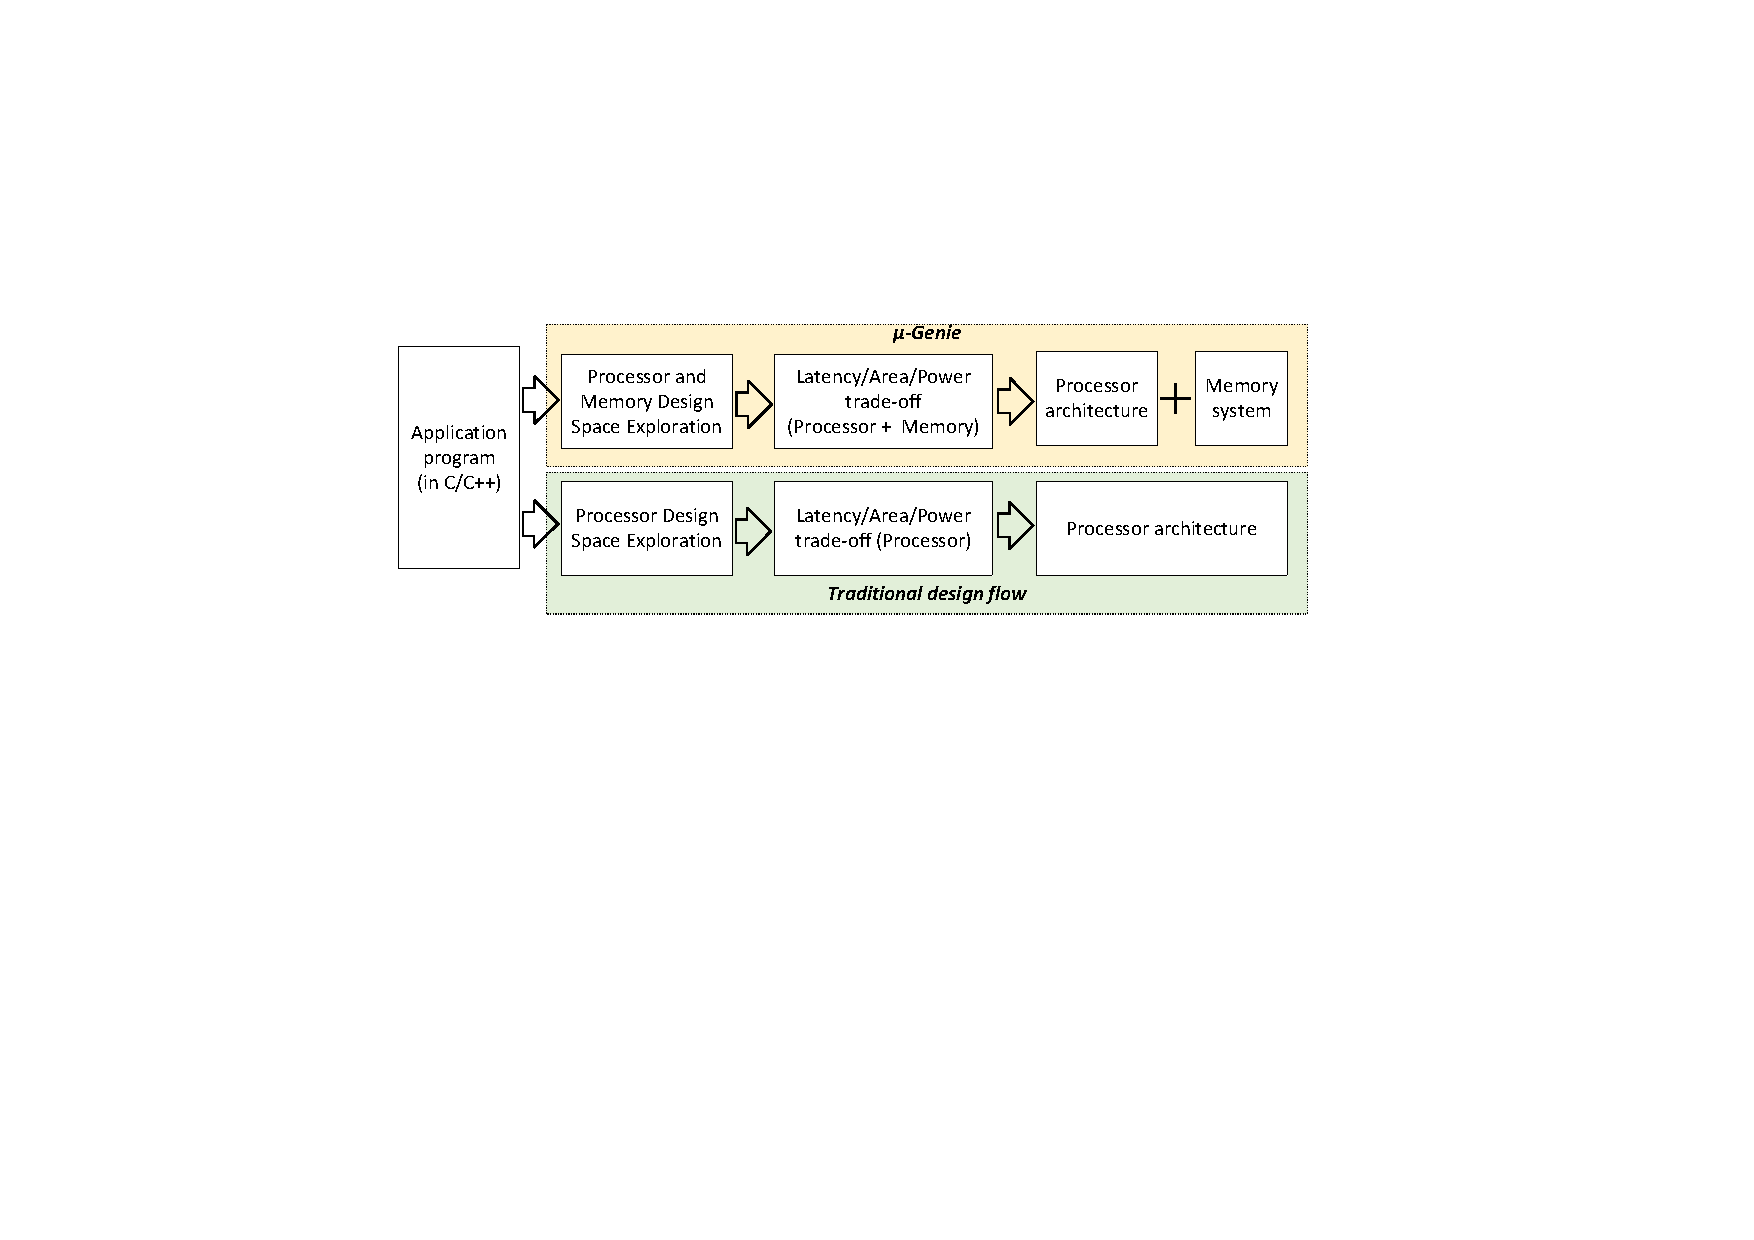
\includegraphics[clip, trim=6cm 10.5cm 6.4cm 5.2cm, width=1.0\linewidth]{images/intro_figure.pdf} %[left down right up ] 
    \caption{Difference between state-of-the-art and the proposed \frameworkname~design flows for custom processor architecture design.}
    \label{fig:intro}
\end{figure}

Our main contributions in this paper are:
\begin{itemize}
\item \frameworkname: An automated framework for memory-aware custom processor architecture design-space exploration and provide different tradeoffs, as shown in Figure~\ref{fig:intro}. The framework supports different kind of memory technologies and configuration of different parameters such as, levels of memory, clock frequency, read/write latency and data width. 
\item A novel spatial processor architecture template that can be configured at design-time (based on the trade-off from the framework) and allows a faster implementation of an application-specific hardware.
\item Case-study demonstrating the effectiveness of the framework for a custom processor design using state-of-the-art MRAM and SRAM for memory system.


%In this work we present \frameworkname, a framework that allows to compare design choices and perform automatic system level design and implementation. We propose a novel memory-driven approach for application-specific hardware design starting from two observations. First, the memory system and the processing system are \textit{interdependent} and therefore they should be \textit{co-designed}. Second, the \textit{data dependencies} of the fixed application impose constaints on the design of both memory and processing systems. Hence, our approach starts from the analysis of an input application and codesigns memory and custom processor, shown in Figure~\ref{fig:intro}. 


\end{itemize}


The rest of this paper is organized as follows. We present the \frameworkname~and describe its modules in section~\ref{sec:framework}. We describe our novel spatial processor architecture in section~\ref{sec:arch_template}. We conclude the paper with three case studies demonstrating the capability of \frameworkname.

